\resizebox{\linewidth}{!}{%
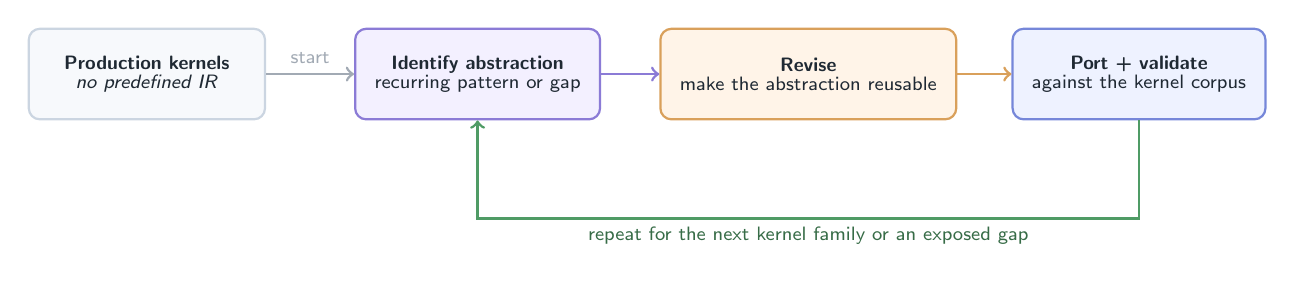
\begin{tikzpicture}[
  font=\sffamily\scriptsize,
  box/.style={rectangle, rounded corners=4pt, draw, line width=0.8pt,
    align=center, inner xsep=7pt, inner ysep=6pt, minimum height=1.15cm},
  flow/.style={->, line width=1.0pt},
  note/.style={font=\sffamily\scriptsize, align=center},
]
\definecolor{irText}{HTML}{1F2933}
\definecolor{irNeutralFill}{HTML}{F7F9FC}
\definecolor{irNeutralBorder}{HTML}{CBD5E1}
\definecolor{irKnowledgeFill}{HTML}{F3F0FF}
\definecolor{irKnowledgeBorder}{HTML}{8B7BD6}
\definecolor{irCandidateFill}{HTML}{FFF4E8}
\definecolor{irCandidateBorder}{HTML}{D9A05B}
\definecolor{irValidationFill}{HTML}{EEF2FF}
\definecolor{irValidationBorder}{HTML}{7687D9}
\definecolor{irSuccessBorder}{HTML}{4F9B65}
\color{irText}

% One external starting point, followed by one repeating three-step loop.
\node[box, fill=irNeutralFill, draw=irNeutralBorder, minimum width=3.0cm]
  (corpus) at (0,0) {\textbf{Production kernels}\\[-1pt]
    \emph{no predefined IR}};
\node[box, fill=irKnowledgeFill, draw=irKnowledgeBorder, minimum width=3.0cm]
  (discover) at (4.2,0) {\textbf{Identify abstraction}\\[-1pt]
    recurring pattern or gap};
\node[box, fill=irCandidateFill, draw=irCandidateBorder, minimum width=3.0cm]
  (revise) at (8.4,0) {\textbf{Revise \cakeir{}}\\[-1pt]
    make the abstraction reusable};
\node[box, fill=irValidationFill, draw=irValidationBorder, minimum width=3.0cm]
  (validate) at (12.6,0) {\textbf{Port + validate}\\[-1pt]
    against the kernel corpus};

\draw[flow, color=irNeutralBorder!80!black]
  (corpus) -- node[note, above] {start} (discover);
\draw[flow, color=irKnowledgeBorder] (discover) -- (revise);
\draw[flow, color=irCandidateBorder] (revise) -- (validate);

% The large return path is the main point of the figure: IR construction never
% terminates at a final box.
\draw[flow, color=irSuccessBorder]
  (validate.south) -- ++(0,-1.25) -| (discover.south);
\node[note, below, color=irSuccessBorder!70!black]
  at (8.4,-1.82) {repeat for the next kernel family or an exposed gap};
\end{tikzpicture}%
}
